\fancyhead[LE]{\fontsize{8.5pt}{10pt}\selectfont\textbf{\textsf{48}}\quad \textbf{\textsf{CHƯƠNG 1}}\quad \textsf{Các hàm số và Mô hình}}
\fancyhead[RO]{\fontsize{8.5pt}{10pt}\selectfont\textsf{MỤC 1.4}\quad \textbf{\textsf{48}}}

\noindent
\begin{minipage}[t]{0.265\textwidth}
    \fontsize{8pt}{10pt}\selectfont
    \vspace{0pt}
    \centering
    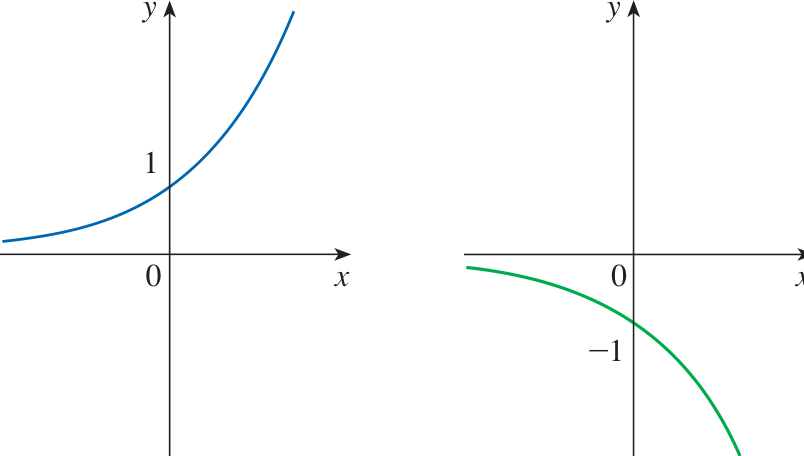
\includegraphics[width=0.92\linewidth]{images/p0083_fig5.png}
    \par\vspace{3pt}
    \makebox[0.92\linewidth][l]{\textbf{\textsf{HÌNH 5}}}
    
    \vspace{1.2em}
    \raggedright
    Ví dụ 2 chỉ ra rằng $y = 2^x$ tăng nhanh hơn $y = x^2$. Để chứng minh hàm số $f(x) = 2^x$ tăng nhanh đến mức nào, hãy cùng thực hiện thí nghiệm tưởng tượng sau đây. Giả sử ta bắt đầu với một mảnh giấy dày một phần nghìn inch và gấp đôi nó lại 50 lần. Mỗi lần gấp đôi, độ dày của mảnh giấy lại tăng gấp hai lần, do đó độ dày của mảnh giấy thu được sẽ là $2^{50}/1000$ inch. Bạn nghĩ độ dày đó lớn đến mức nào? Kết quả tính toán cho thấy nó dài hơn 17 triệu dặm!

    \vspace{1.2em}
    \centering
    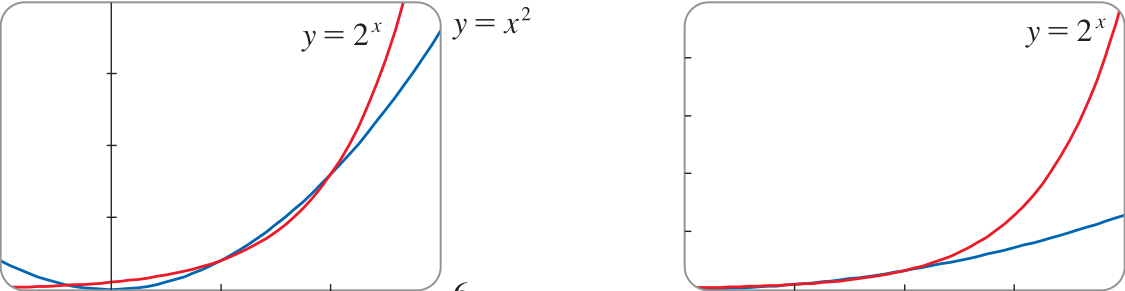
\includegraphics[width=0.92\linewidth]{images/p0083_fig6.png}
    \par\vspace{3pt}
    \makebox[0.92\linewidth][l]{\textbf{\textsf{HÌNH 6}}}
\end{minipage}%
\hfill
\begin{minipage}[t]{0.708\textwidth}
    \fontsize{9.3pt}{13.2pt}\selectfont
    \vspace{0pt}
    \noindent ...lên trên 3 đơn vị để thu được đồ thị của hàm số $y = 3 - 2^x$ trong Hình 5(c). Tập xác định là $\mathbb{R}$ và tập giá trị là $(-\infty, 3)$. \hfill{\color{stewartcyan}$\blacksquare$}

    \vspace{1.2em}
    \noindent\textbf{\textsf{\color{stewartcyan}VÍ DỤ 2}}\quad Sử dụng máy tính bỏ túi có chức năng vẽ đồ thị hoặc máy tính để so sánh hàm số mũ $f(x) = 2^x$ và hàm lũy thừa $g(x) = x^2$. Hàm số nào tăng nhanh hơn khi $x$ lớn?

    \vspace{0.6em}
    \noindent\textbf{\textsf{\color{stewartcyan}LỜI GIẢI}}\quad Hình 6 biểu diễn cả hai hàm số được vẽ trong khung nhìn chữ nhật $[-2, 6] \times [0, 40]$. Ta thấy rằng các đồ thị cắt nhau tại ba điểm, nhưng với $x > 4$, đồ thị của $f(x) = 2^x$ luôn nằm phía trên đồ thị của $g(x) = x^2$. Hình 7 cho một góc nhìn bao quát hơn và chỉ ra rằng với các giá trị lớn của $x$, hàm số mũ $f(x) = 2^x$ tăng nhanh hơn rất nhiều so với hàm lũy thừa $g(x) = x^2$.

    \vspace{0.8em}
    \begin{center}
        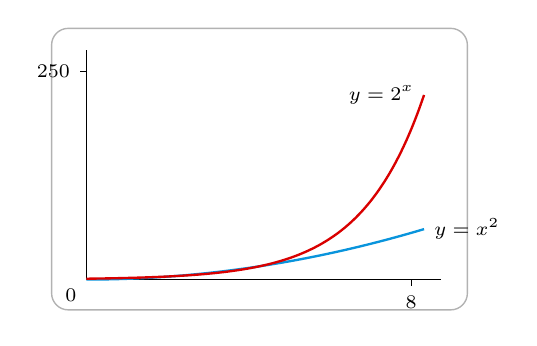
\begin{tikzpicture}[scale=0.55]
            % Khung hiển thị viewing rectangle
            \draw[rounded corners=6pt, line width=0.5pt, gray!60] (-0.8, -0.7) rectangle (8.8, 5.8);
            % Hệ trục tọa độ
            \draw[line width=0.5pt] (0, 0) -- (8.2, 0);
            \draw[line width=0.5pt] (0, 0) -- (0, 5.3);
            % Vạch chia và số
            \node[below left, font=\scriptsize] at (0, 0) {$0$};
            \draw (7.5, 0) -- (7.5, -0.15) node[below, font=\scriptsize] {$8$};
            \draw (0, 4.8) -- (-0.15, 4.8) node[left, font=\scriptsize] {$250$};
            % Đồ thị y = x^2 (màu xanh lam)
            \draw[domain=0:7.8, samples=50, smooth, line width=0.85pt, cyan!80!blue] 
                plot (\x, {(\x*\x)/256 * 4.9}) node[right, font=\scriptsize, black] {$y = x^2$};
            % Đồ thị y = 2^x (màu đỏ)
            \draw[domain=0:7.8, samples=60, smooth, line width=0.85pt, red!85!black] 
                plot (\x, {(2^\x)/256 * 4.9}) node[left, font=\scriptsize, black] {$y = 2^x$};
        \end{tikzpicture}
        \par\vspace{3pt}
        \makebox[\linewidth]{\textbf{\textsf{HÌNH 7}}\hfill{\color{stewartcyan}$\blacksquare$}}
    \end{center}

    \vspace{1.0em}
    \noindent\textbf{\textsf{\large\color{stewartcyan}$\blacksquare$\; \color{black}Ứng dụng của hàm số mũ}}

    \vspace{0.5em}
    \noindent Hàm số mũ xuất hiện rất thường xuyên trong các mô hình toán học của tự nhiên và xã hội. Ở đây, chúng tôi trình bày tóm tắt cách thức nó phát sinh trong việc mô tả sự gia tăng dân số hoặc sự suy giảm tải lượng virus. Trong các chương sau, chúng ta sẽ tiếp tục nghiên cứu sâu hơn về các ứng dụng này và những ứng dụng khác.

    \vspace{0.5em}
    Trước tiên, chúng ta xét một quần thể vi khuẩn trong một môi trường dinh dưỡng đồng nhất. Giả sử rằng bằng việc lấy mẫu quần thể theo những khoảng thời gian nhất định, người ta xác định được rằng quần thể này tăng gấp đôi sau mỗi giờ. Nếu số lượng vi khuẩn tại thời điểm $t$ là $p(t)$, trong đó $t$ được đo bằng giờ, và quần thể ban đầu là $p(0) = 1000$, thì ta có
    \begin{align*}
        p(1) &= 2p(0) = 2 \times 1000 \\
        p(2) &= 2p(1) = 2^2 \times 1000 \\
        p(3) &= 2p(2) = 2^3 \times 1000
    \end{align*}
\end{minipage}